% Global view and the need for better local models
% - Why access higher-order statistical/derivative information
% - Current algorithms are based on gradients, their potential is exhausted
The large number of trainable parameters in deep neural networks imposes
computational constraints on the information that can be made available to
optimization algorithms. Standard machine learning libraries
\citep{abadi2016tensorflow, paszke2019pytorch} mainly provide access to
first-order information in the form of \emph{average} mini-batch gradients. This
is a limitation that complicates the development of novel methods that may
outperform the state-of-the-art: They must use the same objects to remain easy
to implement and use, and to rely on the highly optimized code of those
libraries. There is evidence that this has led to stagnation in the performance
of first-order optimizers \citep{schmidt2021descending}. Here, we thus study how
to provide efficient access to richer information, namely higher-order
derivatives and their distribution across the mini-batch.

\begin{figure}[!tb]
  \centering
  \begin{subfigure}{0.55\linewidth}
    \centering
    \caption{}
    \label{subfig:visual_abstract_1}
  \vspace{-1.3\baselineskip}
  \begin{minipage}[t]{0.33\linewidth}
    \centering
    % load "spectrumdefault{left, center, right}" styles
    % defines the pgfplots styles "spectrumdefault", "spectrumdefaultleft",
% "spectrumdefaultcenter", "spectrumdefaultright"
% pgfplots style "spectrumdefault"
\pgfkeys{/pgfplots/spectrumdefault/.style={
    width=1.38\linewidth,
    height=1.38*1.8\linewidth,
    every axis plot/.append style={line width = 1.5pt},
    tick pos = left,
    xmajorticks = true,
    ymajorticks = true,
    ylabel near ticks,
    xlabel near ticks,
    xtick align = inside,
    ytick align = inside,
    legend cell align = left,
    legend columns = 1,
    legend pos = north west,
    legend style = {
      fill opacity = 0.7,
      text opacity = 1,
      font = \footnotesize,
    },
    xticklabel style = {font = \footnotesize, inner xsep = 0ex},
    xlabel style = {font = \footnotesize},
    axis line style = {black},
    yticklabel style = {font = \footnotesize, inner ysep = 0ex},
    ylabel style = {font = \footnotesize, inner ysep = 0ex},
    title style = {font = \footnotesize, inner ysep = 0ex, yshift = -0.75ex},
    grid = major,
    grid style = {dashed}
  }
}
% pgfplots style for left "spectrumdefaultleft"
\pgfkeys{/pgfplots/spectrumdefaultleft/.style={
    spectrumdefault,
    title=\empty,
    ymax=3e-4,
    xlabel=\phantom{eigenvalues},
  }}
% pgfplots style for center "spectrumdefaultcenter"
\pgfkeys{/pgfplots/spectrumdefaultcenter/.style={
    spectrumdefault,
    ylabel=\empty,
    yticklabels=\empty,
    title=\empty,
    ymax=3e-4,
  }}
% pgfplots style for right "spectrumdefaultright"
\pgfkeys{/pgfplots/spectrumdefaultright/.style={
    spectrumdefault,
    ylabel=\empty,
    yticklabels=\empty,
    title=\empty,
    ymax=3e-4,
    xlabel=\phantom{eigenvalues},
  }}

%%% Local Variables:
%%% mode: latex
%%% TeX-master: "../../thesis"
%%% End:

    % customize "zmystyle" as you wish
    \pgfkeys{/pgfplots/zmystyle/.style={spectrumdefaultleft,
        title={mb, exact}}}
    % This file was created by tikzplotlib v0.9.7.
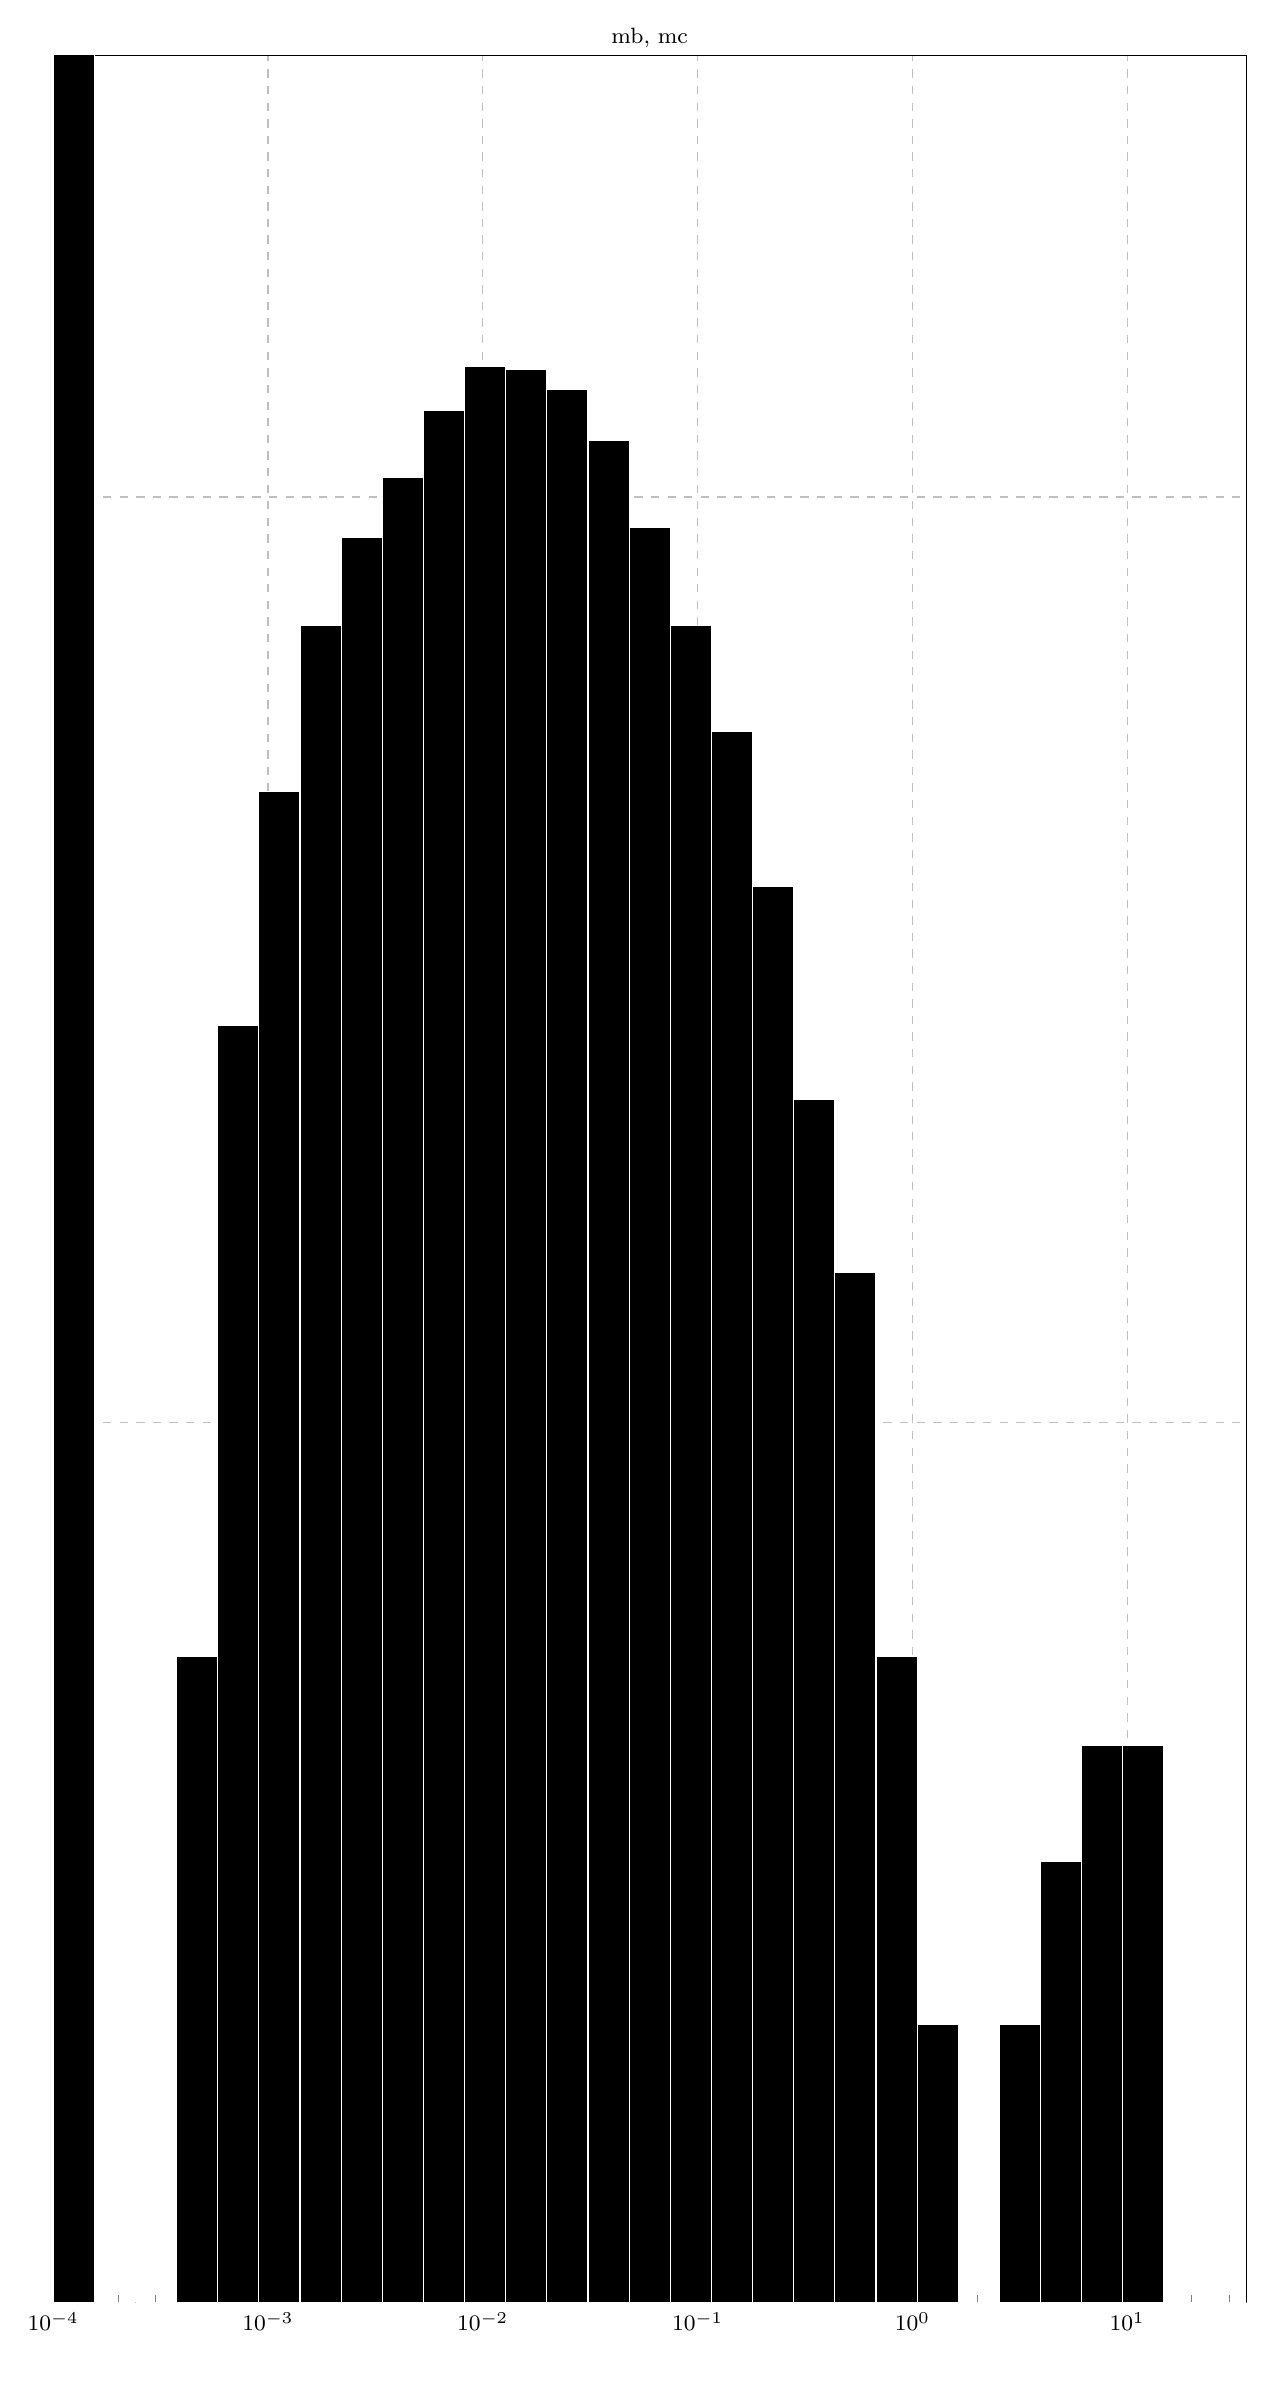
\begin{tikzpicture}

\begin{axis}[
axis line style={white!80!black},
log basis x={10},
tick pos=left,
title={full\_batch\_exact, one\_group, N=128, D=895210},
xlabel={eigenvalues},
xmin=0.0001, xmax=35.8794860839844,
xmode=log,
ylabel={density},
ymin=1.11705508533742e-06, ymax=1,
ymode=log,
zmystyle
]
\draw[draw=white,fill=black] (axis cs:0.0001,1.11705508533742e-06) rectangle (axis cs:0.000155434142340701,0.99871426815899);
\draw[draw=white,fill=black] (axis cs:0.000155434142340701,1.11705508533742e-06) rectangle (axis cs:0.000241597726051892,1.11705508533742e-06);
\draw[draw=white,fill=black] (axis cs:0.000241597726051892,1.11705508533742e-06) rectangle (axis cs:0.000375525353403394,1.11705508533742e-06);
\draw[draw=white,fill=black] (axis cs:0.000375525353403394,1.11705508533742e-06) rectangle (axis cs:0.00058369461233445,5.58528041795857e-06);
\draw[draw=white,fill=black] (axis cs:0.00058369461233445,1.11705508533742e-06) rectangle (axis cs:0.000907260714570931,2.68093507478535e-05);
\draw[draw=white,fill=black] (axis cs:0.000907260714570931,1.11705508533742e-06) rectangle (axis cs:0.00141019291048744,4.80334210778594e-05);
\draw[draw=white,fill=black] (axis cs:0.00141019291048744,1.11705508533742e-06) rectangle (axis cs:0.00219192125576551,7.26086604072757e-05);
\draw[draw=white,fill=black] (axis cs:0.00219192125576551,1.11705508533742e-06) rectangle (axis cs:0.00340699400468264,9.04815617377603e-05);
\draw[draw=white,fill=black] (axis cs:0.00340699400468264,1.11705508533742e-06) rectangle (axis cs:0.00529563191077756,0.000105003294068835);
\draw[draw=white,fill=black] (axis cs:0.00529563191077756,1.11705508533742e-06) rectangle (axis cs:0.00823122004203757,0.000123993251732419);
\draw[draw=white,fill=black] (axis cs:0.00823122004203757,1.11705508533742e-06) rectangle (axis cs:0.0127941262765169,0.000138514984063382);
\draw[draw=white,fill=black] (axis cs:0.0127941262765169,1.11705508533742e-06) rectangle (axis cs:0.0198864404478903,0.000137397927730282);
\draw[draw=white,fill=black] (axis cs:0.0198864404478903,1.11705508533742e-06) rectangle (axis cs:0.0309103181522725,0.000130695589731351);
\draw[draw=white,fill=black] (axis cs:0.0309103181522725,1.11705508533742e-06) rectangle (axis cs:0.0480451879147667,0.000115056801067177);
\draw[draw=white,fill=black] (axis cs:0.0480451879147667,1.11705508533742e-06) rectangle (axis cs:0.0746786257712956,9.27156744040709e-05);
\draw[draw=white,fill=black] (axis cs:0.0746786257712956,1.11705508533742e-06) rectangle (axis cs:0.116076081479435,7.26086604072757e-05);
\draw[draw=white,fill=black] (axis cs:0.116076081479435,1.11705508533742e-06) rectangle (axis cs:0.180421861710252,5.5852815410002e-05);
\draw[draw=white,fill=black] (axis cs:0.180421861710252,1.11705508533742e-06) rectangle (axis cs:0.280437173344456,3.79799140794064e-05);
\draw[draw=white,fill=black] (axis cs:0.280437173344456,1.11705508533742e-06) rectangle (axis cs:0.435895115192459,2.23411254153434e-05);
\draw[draw=white,fill=black] (axis cs:0.435895115192459,1.11705508533742e-06) rectangle (axis cs:0.677529833804408,1.45217310832009e-05);
\draw[draw=white,fill=black] (axis cs:0.677529833804408,1.11705508533742e-06) rectangle (axis cs:1.05311268627626,5.58528041795857e-06);
\draw[draw=white,fill=black] (axis cs:1.05311268627626,1.11705508533742e-06) rectangle (axis cs:1.63689667179461,2.2341114184372e-06);
\draw[draw=white,fill=black] (axis cs:1.63689667179461,1.11705508533742e-06) rectangle (axis cs:2.54429630280743,1.11705508533742e-06);
\draw[draw=white,fill=black] (axis cs:2.54429630280743,1.11705508533742e-06) rectangle (axis cs:3.95470513687488,2.23411141854822e-06);
\draw[draw=white,fill=black] (axis cs:3.95470513687488,1.11705508533742e-06) rectangle (axis cs:6.1469620116051,3.351167751648e-06);
\draw[draw=white,fill=black] (axis cs:6.14696201160511,1.11705508533742e-06) rectangle (axis cs:9.55447768274709,4.46822408474777e-06);
\draw[draw=white,fill=black] (axis cs:9.55447768274709,1.11705508533742e-06) rectangle (axis cs:14.8509204413116,4.46822408485879e-06);
\draw[draw=white,fill=black] (axis cs:14.8509204413116,1.11705508533742e-06) rectangle (axis cs:23.0834008176524,1.11705508533742e-06);
\draw[draw=white,fill=black] (axis cs:23.0834008176524,1.11705508533742e-06) rectangle (axis cs:35.8794860839844,1.11705508533742e-06);
\end{axis}

\end{tikzpicture}

  \end{minipage}
  \hspace{1.9ex}
  \begin{minipage}[t]{0.33\linewidth}
    \centering
    % load "spectrumdefault{left, center, right}" styles
    % defines the pgfplots styles "spectrumdefault", "spectrumdefaultleft",
% "spectrumdefaultcenter", "spectrumdefaultright"
% pgfplots style "spectrumdefault"
\pgfkeys{/pgfplots/spectrumdefault/.style={
    width=1.38\linewidth,
    height=1.38*1.8\linewidth,
    every axis plot/.append style={line width = 1.5pt},
    tick pos = left,
    xmajorticks = true,
    ymajorticks = true,
    ylabel near ticks,
    xlabel near ticks,
    xtick align = inside,
    ytick align = inside,
    legend cell align = left,
    legend columns = 1,
    legend pos = north west,
    legend style = {
      fill opacity = 0.7,
      text opacity = 1,
      font = \footnotesize,
    },
    xticklabel style = {font = \footnotesize, inner xsep = 0ex},
    xlabel style = {font = \footnotesize},
    axis line style = {black},
    yticklabel style = {font = \footnotesize, inner ysep = 0ex},
    ylabel style = {font = \footnotesize, inner ysep = 0ex},
    title style = {font = \footnotesize, inner ysep = 0ex, yshift = -0.75ex},
    grid = major,
    grid style = {dashed}
  }
}
% pgfplots style for left "spectrumdefaultleft"
\pgfkeys{/pgfplots/spectrumdefaultleft/.style={
    spectrumdefault,
    title=\empty,
    ymax=3e-4,
    xlabel=\phantom{eigenvalues},
  }}
% pgfplots style for center "spectrumdefaultcenter"
\pgfkeys{/pgfplots/spectrumdefaultcenter/.style={
    spectrumdefault,
    ylabel=\empty,
    yticklabels=\empty,
    title=\empty,
    ymax=3e-4,
  }}
% pgfplots style for right "spectrumdefaultright"
\pgfkeys{/pgfplots/spectrumdefaultright/.style={
    spectrumdefault,
    ylabel=\empty,
    yticklabels=\empty,
    title=\empty,
    ymax=3e-4,
    xlabel=\phantom{eigenvalues},
  }}

%%% Local Variables:
%%% mode: latex
%%% TeX-master: "../../thesis"
%%% End:

    % customize "zmystyle" as you wish
    \pgfkeys{/pgfplots/zmystyle/.style={spectrumdefaultcenter,
        title={sub, exact}}}
    % This file was created by tikzplotlib v0.9.7.
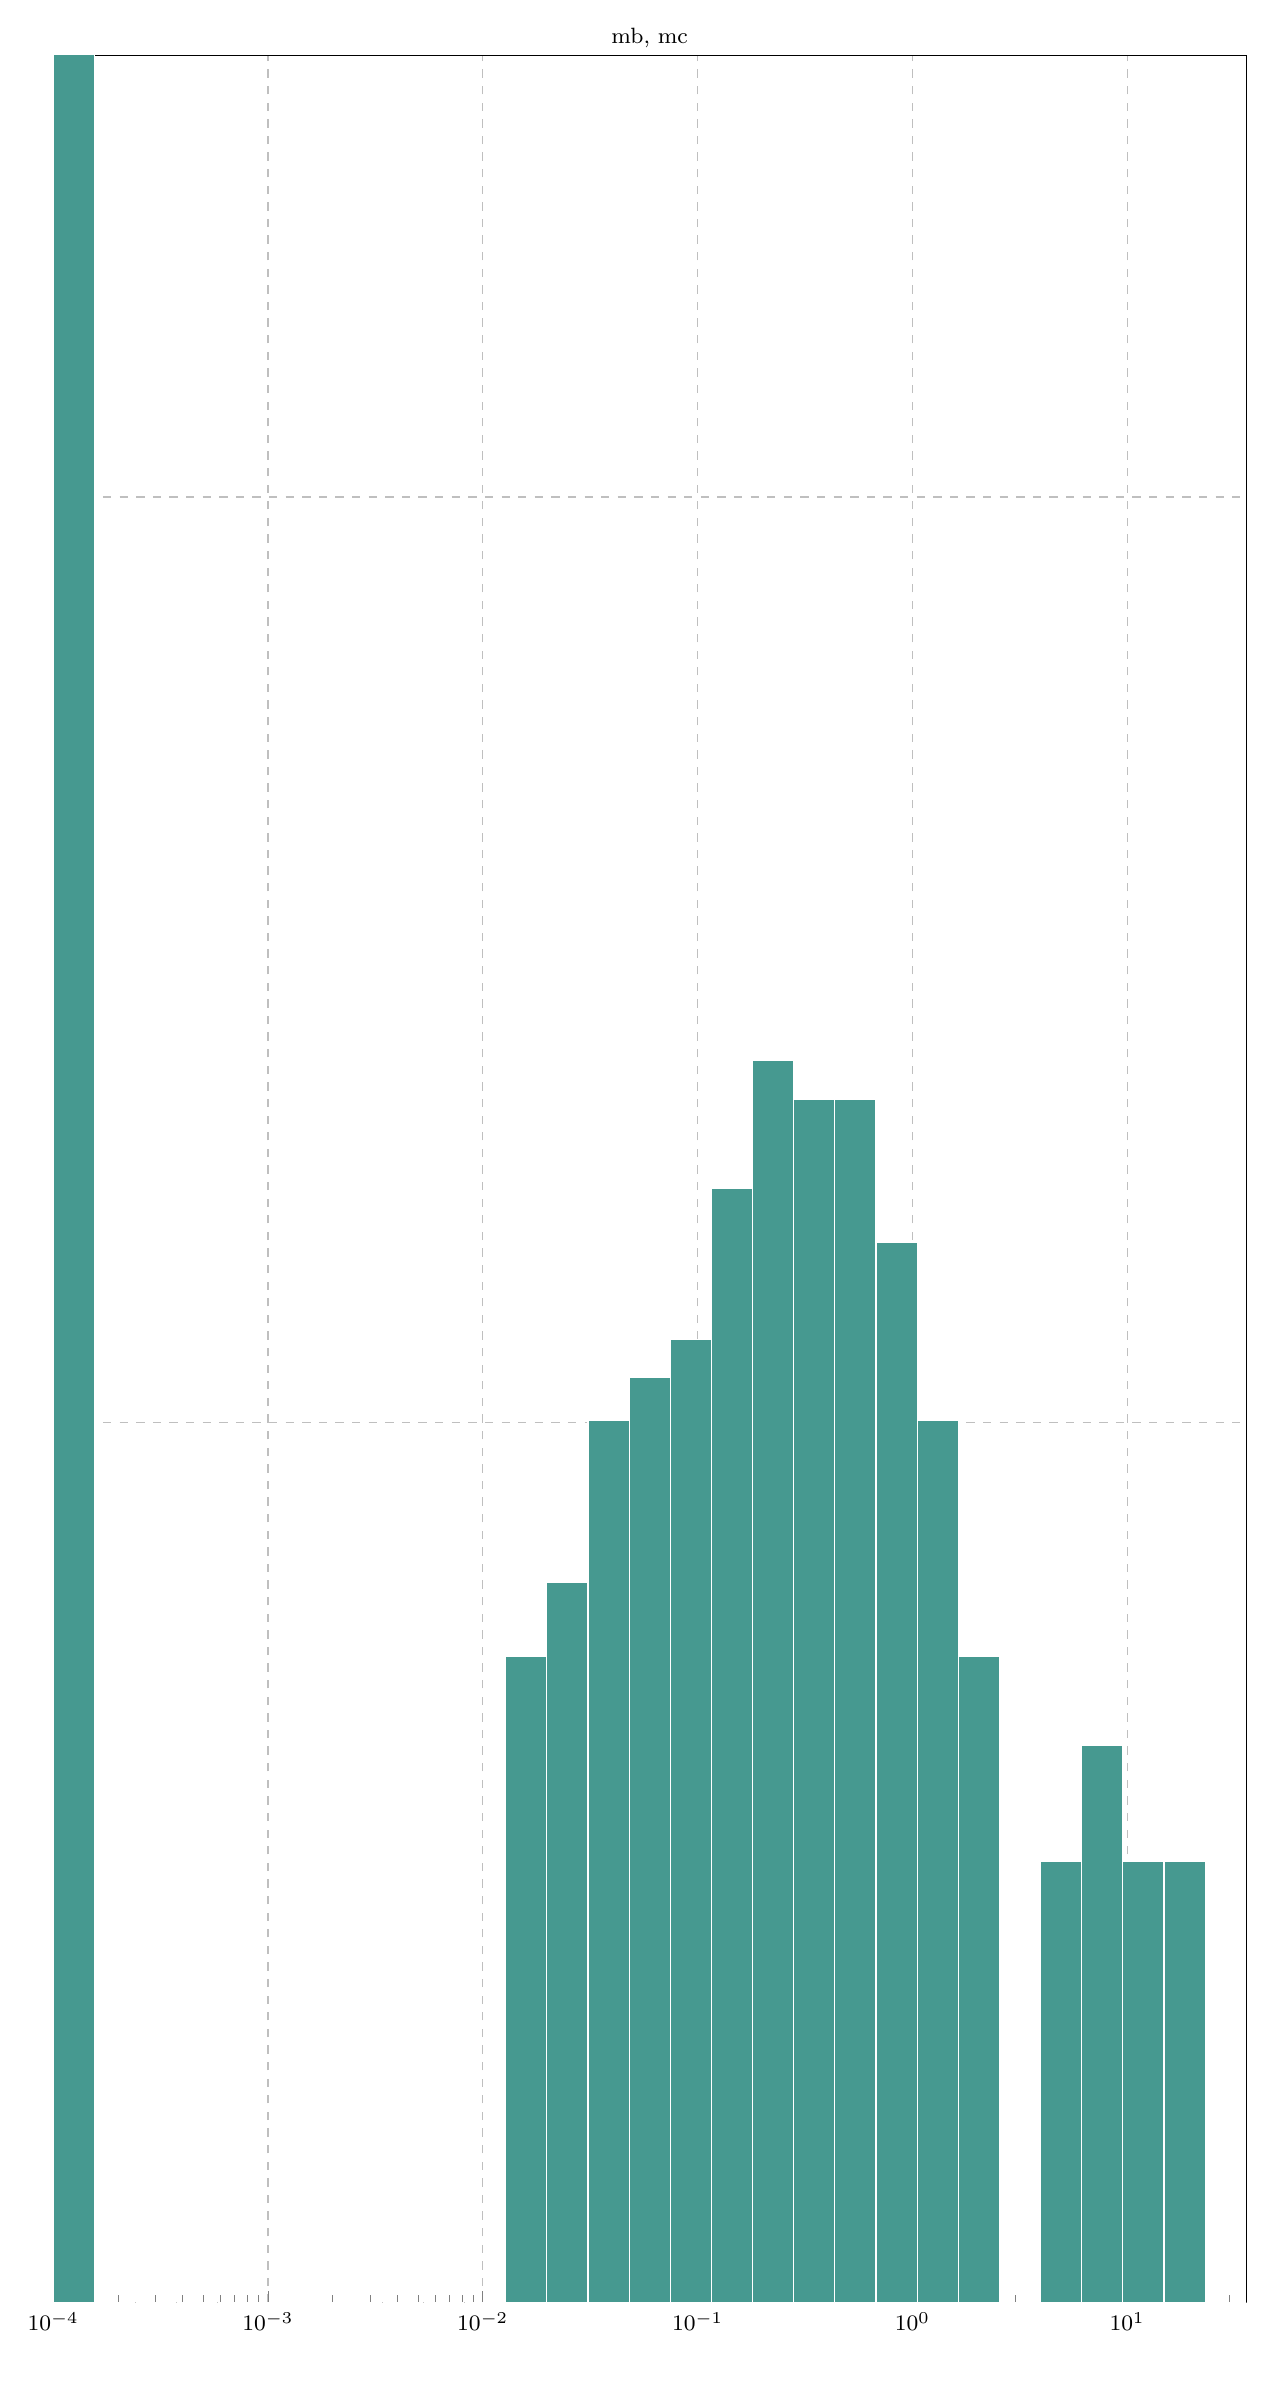
\begin{tikzpicture}

\definecolor{color0}{rgb}{0.274509803921569,0.6,0.564705882352941}

\begin{axis}[
axis line style={white!80!black},
log basis x={10},
tick pos=left,
title={frac\_batch\_exact, one\_group, N=128, D=895210},
xlabel={eigenvalues},
xmin=0.0001, xmax=35.8794860839844,
xmode=log,
ylabel={density},
ymin=1.11705508533742e-06, ymax=1,
ymode=log,
zmystyle
]
\draw[draw=white,fill=color0] (axis cs:0.0001,1.11705508533742e-06) rectangle (axis cs:0.000155434142340701,0.999840260942811);
\draw[draw=white,fill=color0] (axis cs:0.000155434142340701,1.11705508533742e-06) rectangle (axis cs:0.000241597726051892,1.11705508533742e-06);
\draw[draw=white,fill=color0] (axis cs:0.000241597726051892,1.11705508533742e-06) rectangle (axis cs:0.000375525353403394,1.11705508533742e-06);
\draw[draw=white,fill=color0] (axis cs:0.000375525353403394,1.11705508533742e-06) rectangle (axis cs:0.00058369461233445,1.11705508533742e-06);
\draw[draw=white,fill=color0] (axis cs:0.00058369461233445,1.11705508533742e-06) rectangle (axis cs:0.000907260714570931,1.11705508533742e-06);
\draw[draw=white,fill=color0] (axis cs:0.000907260714570931,1.11705508533742e-06) rectangle (axis cs:0.00141019291048744,1.11705508533742e-06);
\draw[draw=white,fill=color0] (axis cs:0.00141019291048744,1.11705508533742e-06) rectangle (axis cs:0.00219192125576551,1.11705508533742e-06);
\draw[draw=white,fill=color0] (axis cs:0.00219192125576551,1.11705508533742e-06) rectangle (axis cs:0.00340699400468264,1.11705508533742e-06);
\draw[draw=white,fill=color0] (axis cs:0.00340699400468264,1.11705508533742e-06) rectangle (axis cs:0.00529563191077756,1.11705508533742e-06);
\draw[draw=white,fill=color0] (axis cs:0.00529563191077756,1.11705508533742e-06) rectangle (axis cs:0.00823122004203757,1.11705508533742e-06);
\draw[draw=white,fill=color0] (axis cs:0.00823122004203757,1.11705508533742e-06) rectangle (axis cs:0.0127941262765169,1.11705508533742e-06);
\draw[draw=white,fill=color0] (axis cs:0.0127941262765169,1.11705508533742e-06) rectangle (axis cs:0.0198864404478903,5.58528041795857e-06);
\draw[draw=white,fill=color0] (axis cs:0.0198864404478903,1.11705508533742e-06) rectangle (axis cs:0.0309103181522725,6.70233675105834e-06);
\draw[draw=white,fill=color0] (axis cs:0.0309103181522725,1.11705508533742e-06) rectangle (axis cs:0.0480451879147667,1.00535057505797e-05);
\draw[draw=white,fill=color0] (axis cs:0.0480451879147667,1.11705508533742e-06) rectangle (axis cs:0.0746786257712956,1.11705620837905e-05);
\draw[draw=white,fill=color0] (axis cs:0.0746786257712956,1.11705508533742e-06) rectangle (axis cs:0.116076081479435,1.22876184168903e-05);
\draw[draw=white,fill=color0] (axis cs:0.116076081479435,1.11705508533742e-06) rectangle (axis cs:0.180421861710252,1.78729000826112e-05);
\draw[draw=white,fill=color0] (axis cs:0.180421861710252,1.11705508533742e-06) rectangle (axis cs:0.280437173344456,2.45752380816539e-05);
\draw[draw=white,fill=color0] (axis cs:0.280437173344456,1.11705508533742e-06) rectangle (axis cs:0.435895115192459,2.23411254152324e-05);
\draw[draw=white,fill=color0] (axis cs:0.435895115192459,1.11705508533742e-06) rectangle (axis cs:0.677529833804408,2.23411254153434e-05);
\draw[draw=white,fill=color0] (axis cs:0.677529833804408,1.11705508533742e-06) rectangle (axis cs:1.05311268627626,1.56387874163006e-05);
\draw[draw=white,fill=color0] (axis cs:1.05311268627626,1.11705508533742e-06) rectangle (axis cs:1.63689667179461,1.00535057505797e-05);
\draw[draw=white,fill=color0] (axis cs:1.63689667179461,1.11705508533742e-06) rectangle (axis cs:2.54429630280743,5.58528041795857e-06);
\draw[draw=white,fill=color0] (axis cs:2.54429630280743,1.11705508533742e-06) rectangle (axis cs:3.95470513687488,1.11705508533742e-06);
\draw[draw=white,fill=color0] (axis cs:3.95470513687488,1.11705508533742e-06) rectangle (axis cs:6.1469620116051,3.351167751648e-06);
\draw[draw=white,fill=color0] (axis cs:6.14696201160511,1.11705508533742e-06) rectangle (axis cs:9.55447768274709,4.46822408485879e-06);
\draw[draw=white,fill=color0] (axis cs:9.55447768274709,1.11705508533742e-06) rectangle (axis cs:14.8509204413116,3.351167751648e-06);
\draw[draw=white,fill=color0] (axis cs:14.8509204413116,1.11705508533742e-06) rectangle (axis cs:23.0834008176524,3.351167751648e-06);
\draw[draw=white,fill=color0] (axis cs:23.0834008176524,1.11705508533742e-06) rectangle (axis cs:35.8794860839844,1.11705508533742e-06);
\end{axis}

\end{tikzpicture}

  \end{minipage}
  \hspace{-3.5ex}
  \begin{minipage}[t]{0.33\linewidth}
    \centering
    % load "spectrumdefault{left, center, right}" styles
    % defines the pgfplots styles "spectrumdefault", "spectrumdefaultleft",
% "spectrumdefaultcenter", "spectrumdefaultright"
% pgfplots style "spectrumdefault"
\pgfkeys{/pgfplots/spectrumdefault/.style={
    width=1.38\linewidth,
    height=1.38*1.8\linewidth,
    every axis plot/.append style={line width = 1.5pt},
    tick pos = left,
    xmajorticks = true,
    ymajorticks = true,
    ylabel near ticks,
    xlabel near ticks,
    xtick align = inside,
    ytick align = inside,
    legend cell align = left,
    legend columns = 1,
    legend pos = north west,
    legend style = {
      fill opacity = 0.7,
      text opacity = 1,
      font = \footnotesize,
    },
    xticklabel style = {font = \footnotesize, inner xsep = 0ex},
    xlabel style = {font = \footnotesize},
    axis line style = {black},
    yticklabel style = {font = \footnotesize, inner ysep = 0ex},
    ylabel style = {font = \footnotesize, inner ysep = 0ex},
    title style = {font = \footnotesize, inner ysep = 0ex, yshift = -0.75ex},
    grid = major,
    grid style = {dashed}
  }
}
% pgfplots style for left "spectrumdefaultleft"
\pgfkeys{/pgfplots/spectrumdefaultleft/.style={
    spectrumdefault,
    title=\empty,
    ymax=3e-4,
    xlabel=\phantom{eigenvalues},
  }}
% pgfplots style for center "spectrumdefaultcenter"
\pgfkeys{/pgfplots/spectrumdefaultcenter/.style={
    spectrumdefault,
    ylabel=\empty,
    yticklabels=\empty,
    title=\empty,
    ymax=3e-4,
  }}
% pgfplots style for right "spectrumdefaultright"
\pgfkeys{/pgfplots/spectrumdefaultright/.style={
    spectrumdefault,
    ylabel=\empty,
    yticklabels=\empty,
    title=\empty,
    ymax=3e-4,
    xlabel=\phantom{eigenvalues},
  }}

%%% Local Variables:
%%% mode: latex
%%% TeX-master: "../../thesis"
%%% End:

    % customize "zmystyle" as you wish
    \pgfkeys{/pgfplots/zmystyle/.style={spectrumdefaultright,
        title={mb, mc}}}
    % This file was created by tikzplotlib v0.9.7.
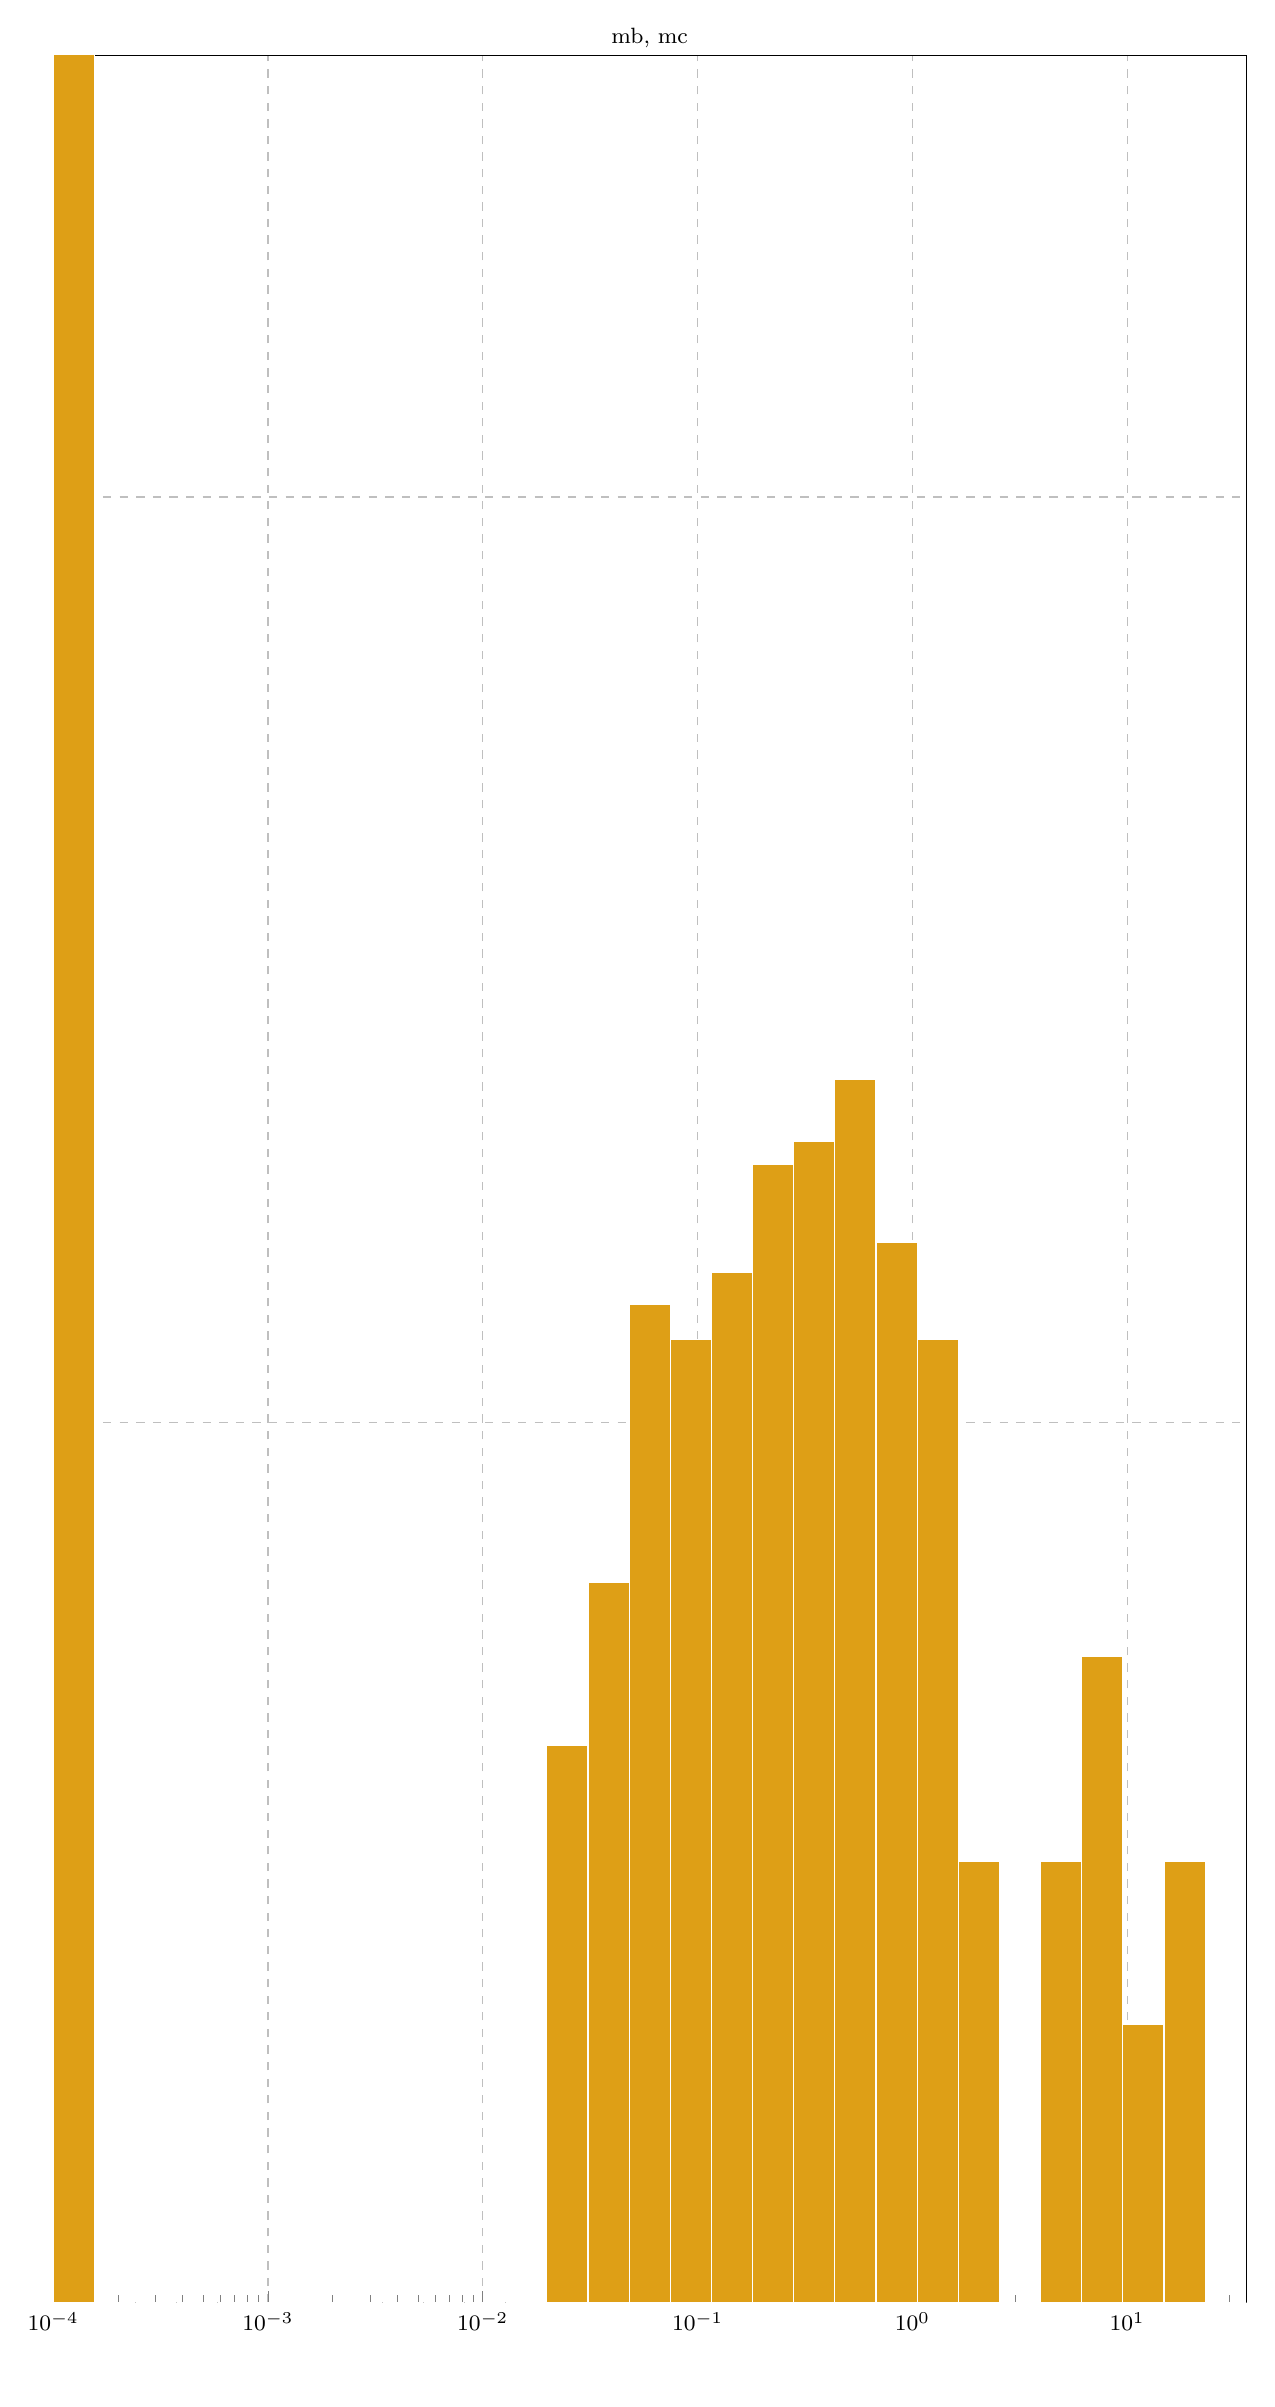
\begin{tikzpicture}

\definecolor{color0}{rgb}{0.870588235294118,0.623529411764706,0.0862745098039216}

\begin{axis}[
axis line style={white!80!black},
log basis x={10},
tick pos=left,
title={full\_batch\_mc, one\_group, N=128, D=895210},
xlabel={eigenvalues},
xmin=0.0001, xmax=35.8794860839844,
xmode=log,
ylabel={density},
ymin=1.11705508533742e-06, ymax=1,
ymode=log,
zmystyle
]
\draw[draw=white,fill=color0] (axis cs:0.0001,1.11705508533742e-06) rectangle (axis cs:0.000155434142340701,0.999858133844141);
\draw[draw=white,fill=color0] (axis cs:0.000155434142340701,1.11705508533742e-06) rectangle (axis cs:0.000241597726051892,1.11705508533742e-06);
\draw[draw=white,fill=color0] (axis cs:0.000241597726051892,1.11705508533742e-06) rectangle (axis cs:0.000375525353403394,1.11705508533742e-06);
\draw[draw=white,fill=color0] (axis cs:0.000375525353403394,1.11705508533742e-06) rectangle (axis cs:0.00058369461233445,1.11705508533742e-06);
\draw[draw=white,fill=color0] (axis cs:0.00058369461233445,1.11705508533742e-06) rectangle (axis cs:0.000907260714570931,1.11705508533742e-06);
\draw[draw=white,fill=color0] (axis cs:0.000907260714570931,1.11705508533742e-06) rectangle (axis cs:0.00141019291048744,1.11705508533742e-06);
\draw[draw=white,fill=color0] (axis cs:0.00141019291048744,1.11705508533742e-06) rectangle (axis cs:0.00219192125576551,1.11705508533742e-06);
\draw[draw=white,fill=color0] (axis cs:0.00219192125576551,1.11705508533742e-06) rectangle (axis cs:0.00340699400468264,1.11705508533742e-06);
\draw[draw=white,fill=color0] (axis cs:0.00340699400468264,1.11705508533742e-06) rectangle (axis cs:0.00529563191077756,1.11705508533742e-06);
\draw[draw=white,fill=color0] (axis cs:0.00529563191077756,1.11705508533742e-06) rectangle (axis cs:0.00823122004203757,1.11705508533742e-06);
\draw[draw=white,fill=color0] (axis cs:0.00823122004203757,1.11705508533742e-06) rectangle (axis cs:0.0127941262765169,1.11705508533742e-06);
\draw[draw=white,fill=color0] (axis cs:0.0127941262765169,1.11705508533742e-06) rectangle (axis cs:0.0198864404478903,1.11705508533742e-06);
\draw[draw=white,fill=color0] (axis cs:0.0198864404478903,1.11705508533742e-06) rectangle (axis cs:0.0309103181522725,4.46822408474777e-06);
\draw[draw=white,fill=color0] (axis cs:0.0309103181522725,1.11705508533742e-06) rectangle (axis cs:0.0480451879147667,6.70233675116937e-06);
\draw[draw=white,fill=color0] (axis cs:0.0480451879147667,1.11705508533742e-06) rectangle (axis cs:0.0746786257712956,1.34046747499901e-05);
\draw[draw=white,fill=color0] (axis cs:0.0746786257712956,1.11705508533742e-06) rectangle (axis cs:0.116076081479435,1.22876184168903e-05);
\draw[draw=white,fill=color0] (axis cs:0.116076081479435,1.11705508533742e-06) rectangle (axis cs:0.180421861710252,1.45217310832009e-05);
\draw[draw=white,fill=color0] (axis cs:0.180421861710252,1.11705508533742e-06) rectangle (axis cs:0.280437173344456,1.8989956415822e-05);
\draw[draw=white,fill=color0] (axis cs:0.280437173344456,1.11705508533742e-06) rectangle (axis cs:0.435895115192459,2.01070127490328e-05);
\draw[draw=white,fill=color0] (axis cs:0.435895115192459,1.11705508533742e-06) rectangle (axis cs:0.677529833804408,2.34581817484432e-05);
\draw[draw=white,fill=color0] (axis cs:0.677529833804408,1.11705508533742e-06) rectangle (axis cs:1.05311268627626,1.56387874163006e-05);
\draw[draw=white,fill=color0] (axis cs:1.05311268627626,1.11705508533742e-06) rectangle (axis cs:1.63689667179461,1.22876184168903e-05);
\draw[draw=white,fill=color0] (axis cs:1.63689667179461,1.11705508533742e-06) rectangle (axis cs:2.54429630280743,3.351167751648e-06);
\draw[draw=white,fill=color0] (axis cs:2.54429630280743,1.11705508533742e-06) rectangle (axis cs:3.95470513687488,1.11705508533742e-06);
\draw[draw=white,fill=color0] (axis cs:3.95470513687488,1.11705508533742e-06) rectangle (axis cs:6.1469620116051,3.351167751648e-06);
\draw[draw=white,fill=color0] (axis cs:6.14696201160511,1.11705508533742e-06) rectangle (axis cs:9.55447768274709,5.58528041795857e-06);
\draw[draw=white,fill=color0] (axis cs:9.55447768274709,1.11705508533742e-06) rectangle (axis cs:14.8509204413116,2.23411141854822e-06);
\draw[draw=white,fill=color0] (axis cs:14.8509204413116,1.11705508533742e-06) rectangle (axis cs:23.0834008176524,3.351167751648e-06);
\draw[draw=white,fill=color0] (axis cs:23.0834008176524,1.11705508533742e-06) rectangle (axis cs:35.8794860839844,1.11705508533742e-06);
\end{axis}

\end{tikzpicture}

  \end{minipage}
  \end{subfigure}
  \hfill
  \begin{subfigure}{0.44\linewidth}
    \centering
    \vspace{-4.7ex}
    \caption{}
    \label{subfig:visual_abstract_2}
    \vspace{-0.8\baselineskip}
    \begin{tikzpicture}
  % PDF Picture. Set the origin to the south west corner
  \node[inner sep=0pt] (pdf_plot) at (0,0){\includegraphics[width=\linewidth]{fig/visual_abstract/vivit_quantities_transparent.pdf}};

  \coordinate (origin) at (pdf_plot.south west);

  % Text
  \node[anchor=south west, inner sep=0pt] at ($ (origin) + (0.25*\linewidth, 0.26*\linewidth)$)
  {$\vtheta_t$};

  \node[anchor=south west, inner sep=0pt] at ($ (origin) + (0.5*\linewidth, 0.26*\linewidth) $)
  {$\textcolor{oo_gelb}{\ve_k}$};

  \node[anchor=south west, inner sep=0pt] at ($ (origin) + (0.85*\linewidth, 0.6*\linewidth) $)
  {$\textcolor{oo_rot}{\gL}$};

  \node[anchor=south west, inner sep=0pt] at ($ (origin) + (0.85*\linewidth, 0.37*\linewidth) $)
  {$\textcolor{oo_blau}{q}$};

  \node[anchor=south west, inner sep=0pt] at ($ (origin) + (0.26*\linewidth, 0.6*\linewidth) $)
  {$\textcolor{oo_gelb}{\mathcal{E}}$};

  \node[anchor=south west, inner sep=0pt, rotate=21] at ($ (origin) + (0.66*\linewidth, 0.035*\linewidth) $)
  {$\textcolor{oo_blau}{\gamma_k} ,\textcolor{oo_blau}{\lambda_k}$};

  \node[anchor=south west, inner sep=0pt, rotate=30] at ($ (origin) + (0.8*\linewidth, -0.02*\linewidth) $)
  {$\textcolor{oo_gruen}{\gamma_{nk}} ,\textcolor{oo_gruen}{\lambda_{nk}}$};
\end{tikzpicture}

%%% Local Variables:
%%% mode: latex
%%% TeX-master: "../main"
%%% End:

    \vspace{-0.5\baselineskip}
  \end{subfigure}

  \vspace{-3.0ex}

  \caption{
  \textbf{Overview of \vivittitle's quantities:}
\textbf{(a)} \ggn eigenvalue distribution of \deepobs' \threecthreed architecture on
\cifarten \cite{schneider2019deepobs}
% ($D = 895,210$, $C = 10$)
for settings with different costs on a mini-batch of size $N = 128$.
From left to right: Exact \ggn,
% on the mini-batch,
exact GGN on a mini-batch fraction,
% ($\nicefrac{1}{8}$, as in \cite{zhang2017blockdiagonal}),
\mc approximation of the \ggn.
% on the mini-batch.
%
\textbf{(b)} Pictorial illustration: Loss function $\textcolor{oo_rot}{\gL}$
from \Cref{eq:objective-function} and quadratic model $\textcolor{oo_blau}{q}$
around $\vtheta_t \in \mathbb{R}^2$ from \Cref{eq:quadratic_model} (both
represented by their contour lines). The low-rank structure provides efficient
access to the \ggn{}'s eigenvectors $\{\textcolor{oo_gelb}{\ve_k}\}$, along
which $\textcolor{oo_blau}{q}$ decouples into one-dimensional parabolas
characterized by the directional derivatives $\textcolor{oo_blau}{\gamma_k},
\textcolor{oo_blau}{\lambda_k}$ and per-sample contributions
$\textcolor{oo_gruen}{\gamma_{nk}}, \textcolor{oo_gruen}{\lambda_{nk}}$
(\Cref{eq:gammas-lambdas}). $\textcolor{oo_gelb}{\mathcal{E}}$ is the \ggn{}'s
top-$1$ eigenspace.}
  \label{fig:visual_abstract}
\end{figure}

%%% Local Variables:
%%% mode: latex
%%% TeX-master: "../main"
%%% End:


% The GGN/Fisher as a practical Hessian approximation
Recent advances in AD \citep{bradbury2018jax, dangel2020backpack} have made such
information more readily accessible through leveraging algebraic structure in
the differentiated loss. We use and extend this functionality to efficiently
access curvature in form of the Hessian's generalized Gauss-Newton (\ggn)
approximation. It offers practical advantages over the Hessian and is
established for training \citep{martens2010deep, martens2015optimizing},
compressing \citep{singh2020woodfisher}, or adding uncertainty to
\citep{ritter2018scalable, ritter2018online, kristiadi2020being} neural
networks.
% It has also been used to investigate the generalization of neural networks
% \citep{jastrzebski2021catastrophic, thomas2020interplay}
It is also linked theoretically to the natural gradient method
\citep{amari1998natural} via the Fisher information matrix \citep[Section
9.2]{martens2014new}.

% Implicit versus explicit
Traditional ways to access curvature fall into two categories. Firstly, repeated
automatic differentiation allows for matrix-free exact multiplication with the
Hessian \citep{pearlmutter1994fast} and \ggn \citep{schraudolph2002fast}.
Iterative linear and eigensolvers can leverage such functionality to compute
Newton steps \citep{martens2010deep, zhang2017blockdiagonal,
  gargiani2020promise} and spectral properties \citep{sagun2017eigenvalues,
  sagun2018empirical, adams2018estimating, ghorbani2019investigation,
  papyan2019spectrum, yao2020pyhessian, granziol2021deep} on arbitrary
architectures thanks to the generality of AD. However, repeated matrix-vector
products are potentially detrimental to performance.

% K-FAC as example for cheap
Secondly, \kfac (Kronecker-factored approximate curvature)
\citep{martens2015optimizing, grosse2016kronecker, botev2017practical,
  martens2018kronecker} constructs an explicit light-weight
representation of the \ggn based on its algebraic Kronecker structure.
% Explain the benefits
The computations are streamlined via gradient backpropagation and the resulting
matrices are cheap to store and invert. This allows \kfac to scale: It has been
used successfully with large mini-batches~\citep{osawa2019large}. One reason for
this efficiency is that \kfac only approximates the \ggn's block diagonal,
neglecting interactions across layers.
% Explain the downsides
Such terms could be useful, however, for applications like uncertainty
quantification with Laplace approximations \citep{ritter2018scalable,
  ritter2018online, kristiadi2020being, daxberger2021laplace} that currently
rely on \kfac. Moreover, due to its specific design for optimization, the
Kronecker representation does not become more accurate with more data. It
remains a simplification, exact only under assumptions unlikely to be met in
practice \citep{martens2015optimizing}. This might be a downside for
applications that depend on a precise curvature proxy.

% Desiderata
Here, we propose \vivit (inspired by $\mV\mV^\top$ in
\Cref{vivit::eq:ggn-factorization}), a curvature model that leverages the \ggn's
low-rank structure. Like \kfac, its representation is computed in parallel with
gradients. But it allows a cost-accuracy trade-off, ranging from the
\emph{exact} \ggn to an approximation that costs a single gradient computation.
Our contributions are:
\begin{itemize}
  % General: Data space versus parameter space
\item We highlight the \ggn's low-rank structure, and the structural limit
  for the inherent curvature information contained in a mini-batch.
  % : Rather than in parameter Gram
  % space, it is best viewed in a significantly smaller Gram space spanned by
  % the data and prediction space size. This expresses a structural limitation
  % how much curvature is contained in a mini-batch.

  % Describe computation
\item We present how to compute various \ggn properties efficiently by
  exploiting this structure (\Cref{vivit::fig:visual_abstract}): The exact eigenvalues,
  eigenvectors, and per-sample directional derivatives. In contrast to other
  methods, these quantities allow modeling curvature noise.

  % Efficient implementation
\item We introduce approximations that allow a flexible trade-off between
  computational cost and accuracy. We also provide a fully-featured efficient
  implementation in \pytorch \citep{paszke2019pytorch} on top of \backpack
  \citep{dangel2020backpack}.

  % Empirical study
\item We empirically demonstrate scalability and efficiency of leveraging the
  \ggn's low-rank structure through benchmarks on different deep neural network
  architectures. Finally, we use \vivit's quantities to study the \ggn, and how
  it is affected by noise, during training.
\end{itemize}

The main focus is demonstrating that many interesting curvature
properties, including uncertainty, can be computed efficiently. Practical
applications of this curvature uncertainty are discussed in
\Cref{vivit::sec:use_cases}.

%%% Local Variables:
%%% mode: latex
%%% TeX-master: "../thesis"
%%% End:
